% Unofficial University of Cambridge Poster Template
% https://github.com/andiac/gemini-cam
% a fork of https://github.com/anishathalye/gemini
% also refer to https://github.com/k4rtik/uchicago-poster

\documentclass[final]{beamer}

% ====================
% Packages
% ====================

\usepackage[T1]{fontenc}
\usepackage{lmodern}
\usepackage[orientation=portrait,size=a0,scale=1.0]{beamerposter}
\usetheme{gemini}
\usecolortheme{nott}
\usepackage{graphicx}
\usepackage{booktabs}
\usepackage{tikz}
\usepackage{pgfplots}
\pgfplotsset{compat=1.14}
\usepackage{anyfontsize}
\usepackage{pythonhighlight}

% ====================
% Lengths
% ====================

% If you have N columns, choose \sepwidth and \colwidth such that
% (N+1)*\sepwidth + N*\colwidth = \paperwidth
\newlength{\sepwidth}
\newlength{\colwidth}
\setlength{\sepwidth}{0.025\paperwidth}
\setlength{\colwidth}{0.45\paperwidth}

\newcommand{\separatorcolumn}{\begin{column}{\sepwidth}\end{column}}

% ====================
% Paths
% ====================
\graphicspath{ {./images/} }

% ====================
% Title
% ====================

\title{SeaIceRT: a python interface for a Delta-Eddington radiative transfer model}

\author{Andrew P. Barrett \inst{1} \and Julienne Stroeve \inst{2} \and Bonnie Light \inst{3} \and Donald Perovich \inst{4}}

\institute[shortinst]{
  \inst{1} National Snow and Ice Data Center
  \samelineand \inst{2} University of Manitoba
  \samelineand \inst{3} Applied Physics Laboratory, University of Washington
  \samelineand \inst{4} University of Dartmouth
}

% ====================
% Footer (optional)
% ====================

\footercontent{
  \href{https://github.com/andypbarrett/seaice\_radiative\_transfer}{https://github.com/andypbarrett/seaice\_radiative\_transfer} \hfill
  Sea Ice Across Temporal and Spatial Scales, Bremerhavn, June 2023 \hfill
  \href{mailto:andrew.barrett@colorado.edu}{andrew.barrett@colorado.edu}}
% (can be left out to remove footer)


% ====================
% Logo (optional)
% ====================

% use this to include logos on the left and/or right side of the header:
\logoright{\includegraphics[height=7cm]{logos/NSIDC_logo_2018_poster.png}}
\logoleft{\includegraphics[height=7cm]{logos/cires_new_logo_large.png}}

% ====================
% Body
% ====================

\begin{document}

% Refer to https://github.com/k4rtik/uchicago-poster
% logo: https://www.cam.ac.uk/brand-resources/about-the-logo/logo-downloads
% \addtobeamertemplate{headline}{}
% {
%     \begin{tikzpicture}[remember picture,overlay]
%       \node [anchor=north west, inner sep=3cm] at ([xshift=-2.5cm,yshift=1.75cm]current page.north west)
%       {\includegraphics[height=7cm]{logos/unott-logo.eps}}; 
%     \end{tikzpicture}
% }

\begin{frame}[t,fragile]
\begin{columns}[t]
\separatorcolumn

\begin{column}{\colwidth}

  \begin{alertblock}{Summary}

    SeaIceRT is a python interface for the single column
    Delta-Eddington sea ice radiative transfer model from the Community Ice
    CodE (CICE) sea ice model used in the NCAR Community Earth System Model
    version 2 (CESM2). The python code provides a simple interface to the
    underlying FORTRAN radiative transfer model. Model parameters and forcing
    variables (ice thickness, snow depth and density, and melt pond depth) can
    be set and explored from an interactive environment such as ipython or
    Jupyter notebooks, as well as incorporated into python scripts to estimate
    under-ice light over periods of time, along transects or for grids for the
    Arctic Ocean. We demonstrate setting up and running the model for several
    transects collected during the MOSAiC cruise and for estimating
    phytoplankton bloom onset for the Arctic Ocean. We hope that the software
    package provides a framework for both simplifying and expanding access to
    these modelling tools. SeaIceRT is open source software. Documentation
    and code can be found at
    https://github.com/andypbarrett/seaice\_radiative\_transfer.

  \end{alertblock}

  \begin{block}{Motivation}

    \begin{figure}[h]
      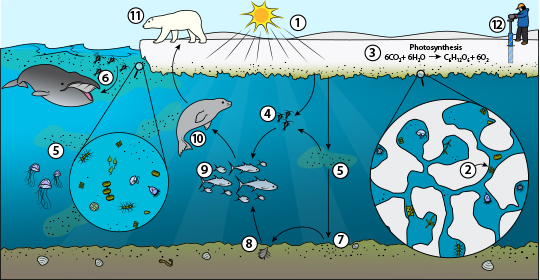
\includegraphics[width=0.75\textwidth]{ecosystemOverview-small}
      \caption{The Arctic Sea Ice Ecosystem https://askabiologist.asu.edu/explore/frozen-life \copyright Arizona Board of Regents ASU Ask A Biologist.}
    \end{figure}
    
    Sunlight transmitted through snow and sea ice to the upper ocean plays an
    important role in regulating biological activity in Polar regions,
    determining the timing of initiations of algal and phytoplankton blooms.
    Measurements of under-ice photosynthetically active radiation (PAR) are
    available from field campaigns and from autonomous buoys. However,
    understanding of the spatial distribution and time evolution of PAR for
    larger regions and over longer time periods requires estimates of light
    transmission through snow and sea ice from radiative transfer models. Even
    intensive and observation rich field campaigns such as MOSAiC can only
    collect measurements from a limited number of measurement points over
    selected periods of time. Radiative transfer models can be used to "fill
    in" gaps in the under ice light field, enabling observations of the
    atmosphere, snow and ice characteristics, oceanography and biology
    collected at distributed locations to be combined.

  \end{block}

  \begin{block}{The Delta-Eddington Radiative Transfer Model}

    The Delta-Eddington (also $\delta$-Eddington) model is a multiple
    scattering parameterization of radiative transfer that uses
    Inherent Optical Properties (IOP) (extinction coefficients, single
    scattering albedo, and asymmetry parameter) for snow, ice and
    other absorbers, along with snow depth, ice thickness and pond
    depth, and incident radiation to calculate albedo, internal
    absorption and light transmission to the upper ocean.  Radiation
    calculations are made for direct and diffuse components of visible
    ($200 \mathrm{nm} - 700 \mathrm{nm}$) and near-infrared ($700
    \mathrm{nm} - 5000 \mathrm{nm}$) solar radiation.  The sea ice
    column consists of snow covered ice, ponded ice or bare ice.  Snow
    and melt ponds are represented as two layers, of which the upper
    layer in both cases is a surface scattering layer.  Sea ice is
    represented as five layers, with the top layer being a ice surface
    scattering layer.  Refraction of incident radiation at pond water
    surfaces and the interface between the ice SSL and underlying ice
    is accounted for by including a refractive (Fresnel) layer.  A
    complete description of the Delta-Eddington model is described in
    \cite{briegleb_delta-eddington_2007}.
    
  \end{block}

  \begin{exampleblock}{Technical details}

    The original program \pyth{1D_SIR_DE} is a stand alone version of
    the CESM3 radiative transfer code and is written in a mixture of
    Fortran 77 and Fortran 95.  Parameters are defined in an input
    text file and results written to an output file.  The motivation
    for writing a Python wrapper for the code, was to allow model runs
    from interactive python interpretters, executable notebooks and
    scripts.  The original Fortran code was modified to allow input
    parameters and results to be passed between compiled Fortran
    routines and the Python wrapper directly, without the need for
    input and output files.  This was done using the \pyth{ctypes}, a
    foreign function library for Python.  The modified fortran code
    was compiled as a shared library.  \pyth{ctypes} data types were
    defined to allow the Python Wrapper code to access data in Fortran
    \pyth{COMMON BLOCKS}.

   
  \end{exampleblock}

\end{column}

\separatorcolumn

\begin{column}{\colwidth}

  \begin{exampleblock}{Running \pyth{SeaIceRT}}

    \pyth{SeaIceRT} is available from the https://github.com/andypbarrett/seaice\_radiative\_transfer github repository.
    Installation instructions along with software requirements are provided there.

    Once installed, SeaIceRT can be run in a Python interpretter, IPython or
    a Jupyter notebook.  I can also be included in other python scripts.  Example
    notebooks are provided in the \pyth{notebooks} folder.

    A simple \pyth{Hello World} example for running \pyth{SeaIceRT} is given below.
    
    \vspace{10mm}
    
    \begin{python}[caption={A \pyth{Hello World} for \pyth{SeaIceRT}}]
      (seaice_radiative_transfer) nsidc-abarrett-442:seaicert$ ipython
      Python 3.7.6 | packaged by conda-forge | (default, Mar  5 2020, 15:27:18) 
      Type 'copyright', 'credits' or 'license' for more information
      IPython 7.17.0 -- An enhanced Interactive Python. Type '?' for help.

      In [1]: from ccsm3_sir_de import SeaIceRT
      In [2]: model = SeaIceRT()
      In [3]: model.run()
      In [4]: model.print_results()
      ----------------------------------------------------------------------
      CCSM3 Sea Ice Delta Eddington calculation
      ----------------------------------------------------------------------
      ----------------------------------------------------------------------
      Visible and near-ir direct and diffuse albedos
      Visible: 0.2 to 0.7 micrometers
      Near-IR: 0.7 to 5.0 micrometers
      ----------------------------------------------------------------------
      Albedo shortwave direct: 0.17
      Albedo shortwave diffuse: 0.19
      Albedo longwave direct: 0.06
      Albedo longwave diffuse: 0.06
       ----------------------------------------------------------------------
      Surface ansorption and Albedos
      ----------------------------------------------------------------------
      Visible solar absorbed by ocean: 27.5656681060791
      Near-IR absorbed by ocean: 0.0
      ----------------------------------------------------------------------
      Surface absorption ad albedos
      ----------------------------------------------------------------------
      Solar vs direct surface irradiance:   0.12 Wm-2
       ----------------------------------------------------------------------
      Snow/Sea ice transmitted flux (Tr fraction) and absorption (Q Wm-2)
      ----------------------------------------------------------------------
      Level      depth Tr_vs  Q_vs   Tr_ni  Q_ni   Q_total
      ----------------------------------------------------------------------
      0 surface                  26.88         68.01  94.89
                 0.000 1.0000        1.0000
      1 pond                     12.76         67.06  79.82
                 0.250 0.9494        0.0130
      2 pond                     12.08          0.93  13.01
                 0.500 0.8625        0.0002
      3 ice                       2.05          0.02   2.07
                 0.050 0.7888        0.0000
      4 ice                      10.84          0.00  10.84
                 0.375 0.6228        0.0000
      5 ice                       9.41          0.00   9.41
                 0.750 0.4730        0.0000
      6 ice                       6.78          0.00   6.78
                 1.125 0.3551        0.0000
      7 ice                       4.61          0.00   4.61
                 1.500 0.2612        0.0000
      8 ocean                    27.57          0.00  27.57
    \end{python}
    
    
  \end{exampleblock}

  \begin{block}{Estimates of Under Ice Sunlight for MOSAiC ice thickness transects}

    We use ice thickness, snow depths and pond depths measured during
    the MOSAiC expedition from Magnaprobe snow and melt pond depth
    measurements from the 2019-2020 MOSAiC expedition
    (https://doi.org/10.1594/PANGAEA.937781) \cite{itkin_sea_2023}.
    Snow depths and pond depths were measured using Magnaprobe
    automatic snow depth probes along established transects regularly
    during the expedition.  Ice thickness was estimated by subtracting
    snow depths from combined snow and ice thicknesses measured using
    the GEM-2 electromagnetic induction instrument.  Ice thicknesses
    and snow depths are available at 1 m to 3 m spacing along
    transects.

    \pyth{SeaIceRT} uses ice thickness, and snow depth or pond depths
    to estimate radiative flux at the ice-ocean interface, along with
    surface albedo, and other variables.

    \begin{figure}[h]
      \includegraphics[width=0.9\textwidth]{radiative_transfer.PS122-5_62-241}
      \caption{Shortwave radiative flux at the ice-ocean interface, surface downwelling shortwave radiation and albedo estimated by \pyth{SeaIceRT}, along with ice thickness, snow depth and pond depth}
    \end{figure}
      

  \end{block}

  
  \begin{block}{References}

    \nocite{*}
    \footnotesize{\bibliographystyle{plain}\bibliography{poster}}

  \end{block}

\end{column}
\separatorcolumn



\end{columns}
\end{frame}

\end{document}
